\documentclass[11pt,a4paper]{article}

\usepackage[margin=2.5cm]{geometry}
\usepackage[T1]{fontenc}
\usepackage{lmodern}
\usepackage{microtype}
\usepackage{amsmath}
\usepackage{booktabs,tabularx,array,longtable}
\usepackage{xcolor}
\usepackage{graphicx}
\usepackage{enumitem}
\usepackage{caption}
\usepackage{fancyhdr}
\usepackage{tikz}
\usetikzlibrary{arrows.meta,shapes.geometric,fit,calc,backgrounds}
\usepackage[hidelinks]{hyperref}

\captionsetup{font=small,labelfont=bf}
\setlist{itemsep=2pt,topsep=4pt}
\setlength{\parindent}{0pt}
\setlength{\parskip}{6pt}
\renewcommand{\arraystretch}{1.2}

\pagestyle{fancy}
\fancyhf{}
\fancyhead[L]{\small Dhuno: motivation, use cases and roadmap}
\fancyhead[R]{\small IIIT Bhubaneswar}
\fancyfoot[C]{\small\thepage}
\renewcommand{\headrulewidth}{0.3pt}

% ---- fill these in once ----
\newcommand{\rollA}{[Roll No.]}
\newcommand{\rollB}{[Roll No.]}
\newcommand{\rollC}{[Roll No.]}
\newcommand{\supervisor}{[Supervisor Name]}

% ---- status labels ----
\newcommand{\done}{\textcolor{green!45!black}{\textbf{Done}}}
\newcommand{\partialstatus}{\textcolor{orange!80!black}{\textbf{Partial}}}
\newcommand{\planned}{\textcolor{red!60!black}{\textbf{Planned}}}

% ---- diagram styles ----
\tikzset{
  blk/.style={draw=#1!70!black, fill=#1!12, rounded corners=3pt, align=center,
              font=\footnotesize, inner sep=4pt},
  db/.style={cylinder, shape border rotate=90, aspect=0.25, draw=orange!70!black,
             fill=orange!12, align=center, font=\footnotesize,
             minimum width=2.3cm, minimum height=1.2cm},
  flow/.style={-{Stealth[length=2.2mm]}, thick, gray!70!black},
  flow2/.style={{Stealth[length=2.2mm]}-{Stealth[length=2.2mm]}, thick, gray!70!black},
  lab/.style={font=\scriptsize, fill=white, inner sep=1.5pt},
  grp/.style={draw=#1!50, dashed, rounded corners=5pt, inner sep=8pt},
}

\begin{document}

% ======================================================================
%  TITLE PAGE
% ======================================================================
\begin{titlepage}
\centering
\vspace*{1.5cm}
\IfFileExists{../Frontend/public/logo.png}{%
  
\includegraphics[width=3cm]{../Frontend/public/logo.png}\par\vspace{1cm}}{}
{\Huge\bfseries Dhuno\par}
\vspace{0.6cm}
{\Large Why we built it, where it fits,\\ and where it goes next\par}
\vspace{0.8cm}
{\large Use cases, implementation status and roadmap\\
\small Companion to the B.Tech project report\par}
\vspace{2cm}
{\large
\begin{tabular}{rl}
\textbf{Nabin Agrawal} & \rollA \\
\textbf{Kumar Vanshaj} & \rollB \\
\textbf{Parlin Kant Goyal} & \rollC \\
\end{tabular}\par}
\vspace{1.2cm}
Under the supervision of\\
\textbf{\supervisor}
\vfill
Department of Computer Science and Engineering\\
\textbf{International Institute of Information Technology, Bhubaneswar}\\[4pt]
\today
\end{titlepage}

% ======================================================================
%  ABSTRACT
% ======================================================================
\begin{abstract}
\noindent
Dhuno is a web platform in which many people hear the same song at the same moment,
each through their own device. The main project report explains how it is built. This
companion document explains why it was built and where it is going. Our central idea is
that the phones people already carry can replace much of the sound hardware needed at a
concert, on a car trip or at a small party, and that personal playback also keeps sound
close to the listener instead of spreading it into the surroundings. We map these
scenarios to the current implementation (server-authoritative rooms, host or DJ control,
location-based discovery, offline downloads), state plainly what is finished and what is
not, and set out the work needed to make the scenarios dependable: clock-offset
compensation, an offline nearby mode that works without internet, scaling for large
audiences, and a measured evaluation.
\end{abstract}

\setcounter{tocdepth}{1}
\tableofcontents
\newpage

% ======================================================================
\section{Introduction}
% ======================================================================
The main report~\cite{main} (\emph{Dhuno: A Real-Time Synchronized Music Streaming Platform with
Host-Controlled Listening Rooms}) documents the problem statement, literature, design and
implementation. It frames the project mostly around people who are in different places and
want to hear the same song together.

This document widens that framing. We also want Dhuno to work when people are in the
\emph{same} place: a crowd at a concert, friends in a car, a room party with too few
speakers. These settings change what the system must guarantee, so they matter for the
design and for the future work. The document is organised as follows.

\begin{itemize}
  \item Section~\ref{sec:why} explains why we thought of the project.
  \item Section~\ref{sec:usecases} describes the target use cases.
  \item Section~\ref{sec:design} shows how the current design supports them.
  \item Section~\ref{sec:done} lists what is implemented so far.
  \item Section~\ref{sec:gaps} states honestly where the system falls short of the use cases.
  \item Sections~\ref{sec:future}--\ref{sec:roadmap} describe future work, how we will
        measure it, and the order we plan to do it in.
\end{itemize}

% ======================================================================
\section{Why we thought of Dhuno}\label{sec:why}
% ======================================================================
\subsection{Listening became solitary, but enjoying music is still social}
Streaming made music instantly available, but it also made listening a private activity.
Sharing a song in person still means passing one earbud or pointing a phone at a friend.
Sharing at a distance means a video call with a phone held near a speaker.

\subsection{Shared listening needs hardware that is often missing}
Playing music for a group normally depends on one device doing all the work.
\begin{itemize}
  \item At a small party, in a hostel room or on a trip, there is often \textbf{no speaker
        at all}, or one small speaker that is too quiet for the whole group.
  \item A single speaker is a \textbf{single point of failure}: if its battery dies or the
        Bluetooth link drops, the music stops for everyone.
  \item A concert needs a large sound system, which is costly to hire, transport and set up.
\end{itemize}

\subsection{Sound spreads to people who did not ask for it}
A loud shared speaker is heard by everyone nearby, including neighbours, people studying
or sleeping, and passers-by. This is ordinary noise pollution. If each listener hears the
music through their own earphones or at their own volume, the sound stays near the
listener and the surroundings stay quiet. Venues sometimes use this idea for ``silent''
events, but it normally needs dedicated transmitters and headsets.

\subsection{The devices are already there}
Everyone in the room already carries a phone. That phone is a speaker, an audio output for
earphones, a screen for controls, and a network node. Our idea is to treat the crowd's
devices as the sound system: one person (or a performer) is the \emph{host}, and every
other device plays the same track at the same moment.

\begin{figure}[htbp]
\centering
\resizebox{\linewidth}{!}{%
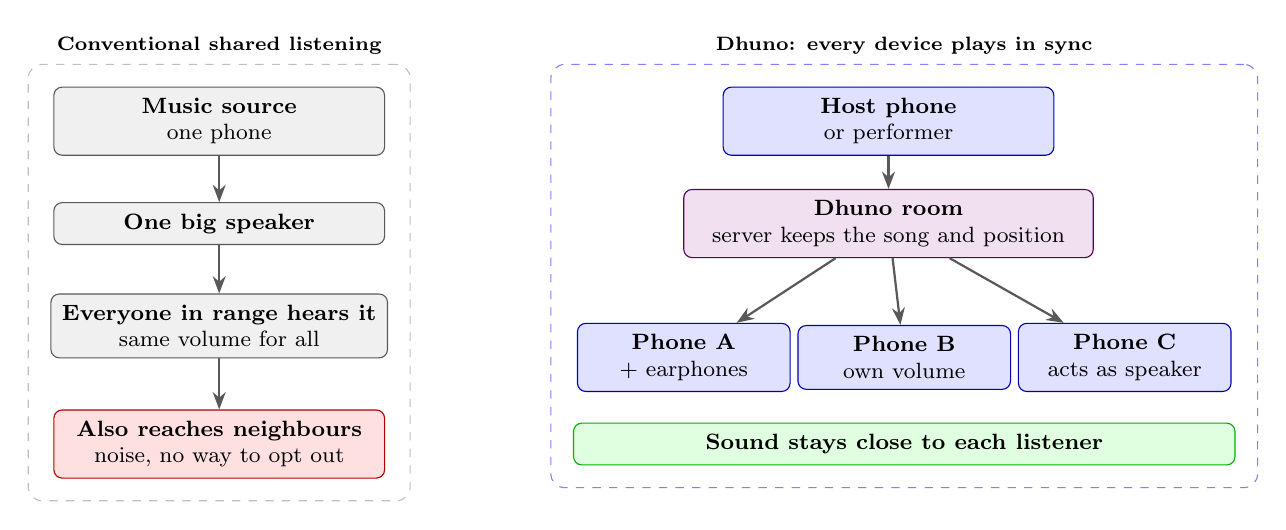
\begin{tikzpicture}[font=\footnotesize]
% left panel
\node[blk=gray, minimum width=4.2cm] (a1) at (3,3.2) {\textbf{Music source}\\one phone};
\node[blk=gray, minimum width=4.2cm] (a2) at (3,1.9) {\textbf{One big speaker}};
\node[blk=gray, minimum width=4.2cm] (a3) at (3,0.6) {\textbf{Everyone in range hears it}\\same volume for all};
\node[blk=red, minimum width=4.2cm] (a4) at (3,-0.9) {\textbf{Also reaches neighbours}\\noise, no way to opt out};
\draw[flow] (a1)--(a2); \draw[flow] (a2)--(a3); \draw[flow] (a3)--(a4);
\begin{scope}[on background layer]
\node[grp=gray, fit=(a1)(a2)(a3)(a4), label={[font=\scriptsize\bfseries]above:Conventional shared listening}] {};
\end{scope}
% right panel
\node[blk=blue, minimum width=4.2cm] (b1) at (11.5,3.2) {\textbf{Host phone}\\or performer};
\node[blk=violet, minimum width=5.2cm] (b2) at (11.5,1.9) {\textbf{Dhuno room}\\server keeps the song and position};
\node[blk=blue, minimum width=2.7cm] (b3) at (8.9,0.2) {\textbf{Phone A}\\+ earphones};
\node[blk=blue, minimum width=2.7cm] (b4) at (11.7,0.2) {\textbf{Phone B}\\own volume};
\node[blk=blue, minimum width=2.7cm] (b5) at (14.5,0.2) {\textbf{Phone C}\\acts as speaker};
\node[blk=green, minimum width=8.4cm] (b6) at (11.7,-0.9) {\textbf{Sound stays close to each listener}};
\draw[flow] (b1)--(b2);
\draw[flow] (b2)--(b3); \draw[flow] (b2)--(b4); \draw[flow] (b2)--(b5);
\begin{scope}[on background layer]
\node[grp=blue, fit=(b1)(b2)(b3)(b4)(b5)(b6), label={[font=\scriptsize\bfseries]above:Dhuno: every device plays in sync}] {};
\end{scope}
\end{tikzpicture}}
\caption{The core idea: replace one shared sound source with many synchronized personal ones.}
\label{fig:idea}
\end{figure}

\subsection{Gaps in existing products}
The main report reviews Spotify Jam~\cite{jam}, Apple SharePlay and the discontinued Turntable.fm
and finds five gaps: ecosystem lock-in, weak host authority, no local discovery, fragile
room state, and separated listener and creator tools. Dhuno answers these in a browser,
with a host who controls the room and an artist area in the same app. None of those
products is designed around the in-person scenarios below.

% ======================================================================
\section{Use cases}\label{sec:usecases}
% ======================================================================
\begin{figure}[htbp]
\centering
\resizebox{0.95\linewidth}{!}{%
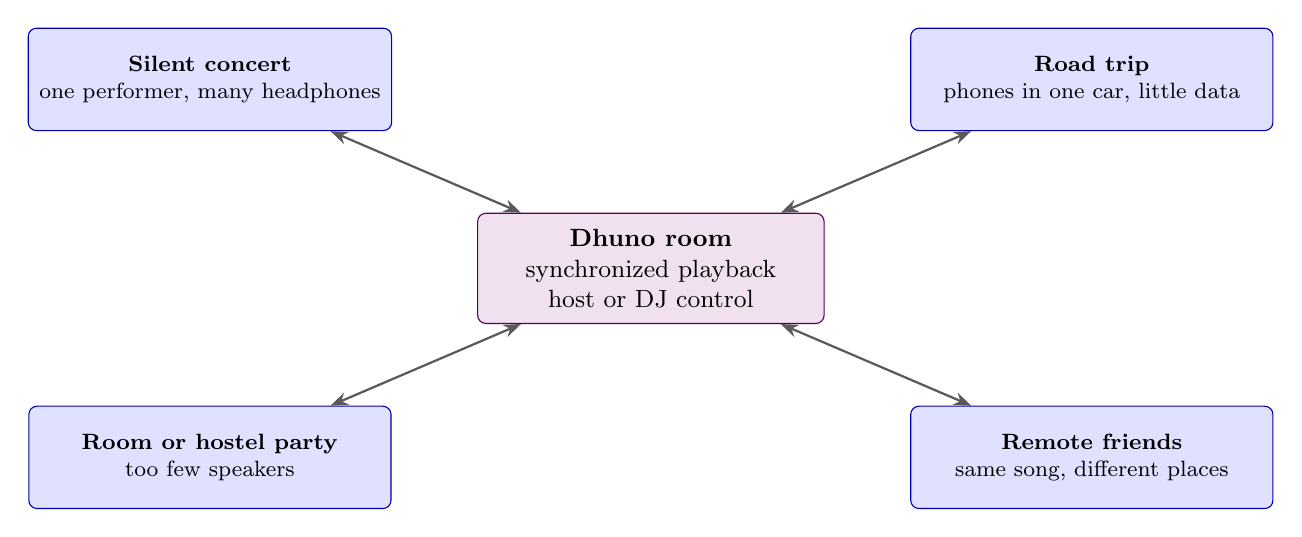
\begin{tikzpicture}[font=\footnotesize]
\node[blk=violet, minimum width=4.4cm, minimum height=1.4cm, font=\small] (core) at (0,0)
  {\textbf{Dhuno room}\\synchronized playback\\host or DJ control};
\node[blk=blue, minimum width=4.6cm, minimum height=1.3cm] (u1) at (-5.6,2.4) {\textbf{Silent concert}\\one performer, many headphones};
\node[blk=blue, minimum width=4.6cm, minimum height=1.3cm] (u2) at (5.6,2.4) {\textbf{Road trip}\\phones in one car, little data};
\node[blk=blue, minimum width=4.6cm, minimum height=1.3cm] (u3) at (-5.6,-2.4) {\textbf{Room or hostel party}\\too few speakers};
\node[blk=blue, minimum width=4.6cm, minimum height=1.3cm] (u4) at (5.6,-2.4) {\textbf{Remote friends}\\same song, different places};
\draw[flow2] (core) -- (u1); \draw[flow2] (core) -- (u2);
\draw[flow2] (core) -- (u3); \draw[flow2] (core) -- (u4);
\end{tikzpicture}}
\caption{One room model, four settings.}
\label{fig:usecases}
\end{figure}

\subsection{UC1: Silent concert}
A performer or DJ is the host. The audience wears headphones and joins the room on their
phones, so everyone hears the same set while the venue itself stays quiet. This suits
places where loud amplified sound is not allowed or not wanted, such as a campus lawn at
night, a library event or a residential area. Dhuno's DJ mode already lets the host hand
control to a chosen DJ. The audience can chat and react in the room. Today the set must
come from tracks uploaded to Dhuno, not from live instruments.

\subsection{UC2: Car or road trip}
Passengers in a small car often have no speaker that suits everyone, and mobile data is
unreliable on highways. The driver or a passenger hosts; others follow with earphones, or
the phones themselves act as speakers. This case depends on songs being downloaded
beforehand and on the group being able to connect without internet.

\subsection{UC3: Room or hostel party}
Ten people, one weak speaker. Several phones placed around the room can all play the same
song, which together act as a distributed speaker system. If people want to stay quiet for
neighbours, they can use earphones instead. The host controls the queue, and guests add
songs and vote to skip.

\subsection{UC4: Remote friends}
The original scenario: friends in different places join one room over the internet. This
is what the current release serves best.

\begin{table}[htbp]
\centering
\caption{Scenarios compared. ``Sync need'' is how closely devices must agree.}
\label{tab:scenarios}
\footnotesize
\begin{tabularx}{\textwidth}{@{}l>{\raggedright\arraybackslash}X>{\raggedright\arraybackslash}X>{\raggedright\arraybackslash}X@{}}
\toprule
\textbf{Scenario} & \textbf{Who and where} & \textbf{Network} & \textbf{Sync need} \\
\midrule
UC1 Silent concert & One performer, many listeners with headphones, outdoors or in a hall
  & Crowded mobile or venue Wi-Fi
  & Low between listeners (each hears only their own headphones). Higher against a visible performer. \\
UC2 Road trip & 2 to 5 people in one car
  & Often no data
  & High if phones act as speakers, low with earphones. \\
UC3 Room party & 5 to 20 people, several phones as speakers
  & Home Wi-Fi, or none
  & High: a few tens of milliseconds of difference between nearby speakers is heard as echo. \\
UC4 Remote friends & Any number, anywhere
  & Internet
  & Moderate: each listener hears only their own device. \\
\bottomrule
\end{tabularx}
\end{table}

The table shows the important pattern. \textbf{When listeners are close together and their
devices act as speakers, synchronization must be much tighter than for remote friends,
and the system should not depend on the internet.} The main report explicitly targets
``perceptually acceptable synchronization for casual group listening''. The in-person
scenarios push beyond that target, which drives the future work in Section~\ref{sec:future}.

% ======================================================================
\section{How the current design supports these scenarios}\label{sec:design}
% ======================================================================
\subsection{Architecture}
Dhuno is a three-tier web application with a separate real-time channel
(Figure~\ref{fig:arch}). The browser runs a React single-page app. An Express server
handles REST calls, and a Socket.IO gateway~\cite{socketio}, built on WebSockets~\cite{ws},
on the same HTTP server keeps live rooms in sync. MongoDB stores durable data, Redis~\cite{redis}
holds fast-changing state, and Cloudinary stores audio and images.

\begin{figure}[htbp]
\centering
\resizebox{\linewidth}{!}{%
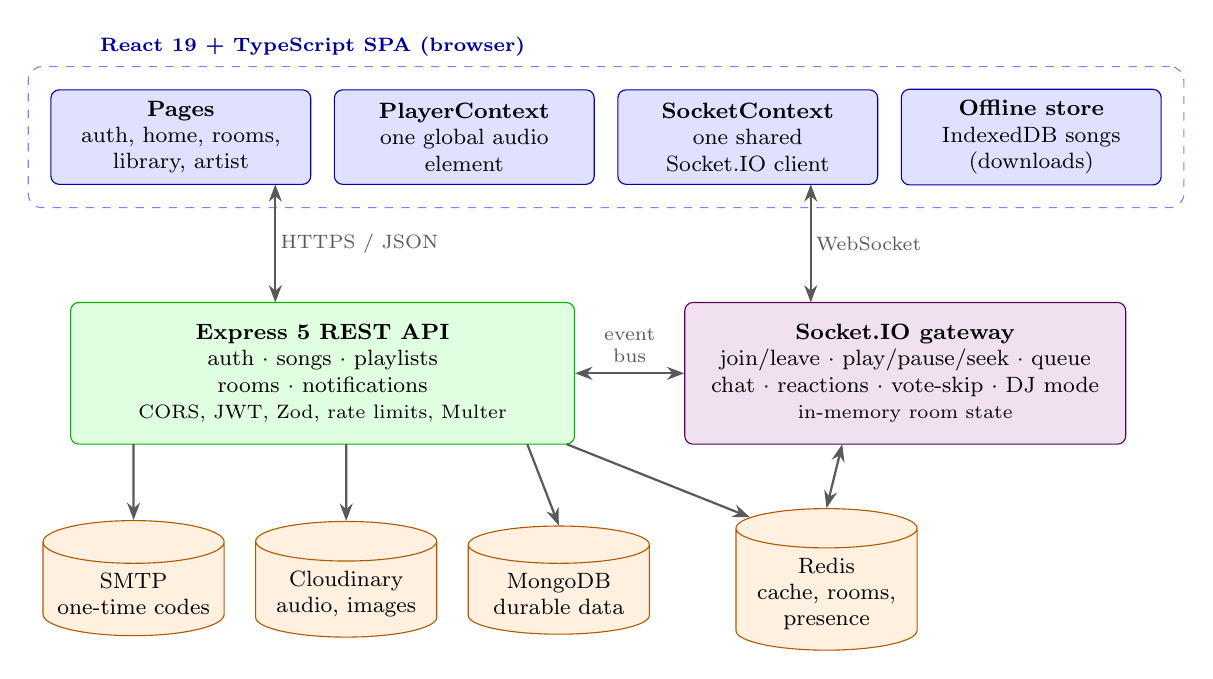
\begin{tikzpicture}[font=\footnotesize]
% client
\node[blk=blue, minimum width=3.3cm, minimum height=1.2cm] (pages) at (1.8,6) {\textbf{Pages}\\auth, home, rooms,\\library, artist};
\node[blk=blue, minimum width=3.3cm, minimum height=1.2cm] (player) at (5.4,6) {\textbf{PlayerContext}\\one global audio\\element};
\node[blk=blue, minimum width=3.3cm, minimum height=1.2cm] (sockctx) at (9.0,6) {\textbf{SocketContext}\\one shared\\Socket.IO client};
\node[blk=blue, minimum width=3.3cm, minimum height=1.2cm] (idb) at (12.6,6) {\textbf{Offline store}\\IndexedDB songs\\(downloads)};
\begin{scope}[on background layer]
\node[grp=blue, fit=(pages)(player)(sockctx)(idb), label={[font=\scriptsize\bfseries,text=blue!60!black]above left:React 19 + TypeScript SPA (browser)}] {};
\end{scope}
% backend
\node[blk=green, minimum width=6.4cm, minimum height=1.8cm] (rest) at (3.6,3) {\textbf{Express 5 REST API}\\auth $\cdot$ songs $\cdot$ playlists\\rooms $\cdot$ notifications\\{\scriptsize CORS, JWT, Zod, rate limits, Multer}};
\node[blk=violet, minimum width=5.6cm, minimum height=1.8cm] (sock) at (11.0,3) {\textbf{Socket.IO gateway}\\join/leave $\cdot$ play/pause/seek $\cdot$ queue\\chat $\cdot$ reactions $\cdot$ vote-skip $\cdot$ DJ mode\\{\scriptsize in-memory room state}};
\draw[flow2] (rest.east) -- (sock.west) node[midway, above, font=\scriptsize, align=center]{event\\bus};
% data
\node[db] (smtp) at (1.2,0.2) {SMTP\\one-time codes};
\node[db] (cloud) at (3.9,0.2) {Cloudinary\\audio, images};
\node[db] (mongo) at (6.6,0.2) {MongoDB\\durable data};
\node[db] (redis) at (10.0,0.2) {Redis\\cache, rooms,\\presence};
% edges
\draw[flow2] (3.0,5.4) -- (3.0,3.9) node[midway, lab, right]{HTTPS / JSON};
\draw[flow2] (9.8,5.4) -- (9.8,3.9) node[midway, lab, right]{WebSocket};
\draw[flow] (1.2,2.1) -- (smtp.north);
\draw[flow] (3.9,2.1) -- (cloud.north);
\draw[flow] (6.2,2.1) -- (mongo.north);
\draw[flow] (6.7,2.1) -- (redis.north west);
\draw[flow2] (10.2,2.1) -- (redis.north);
\end{tikzpicture}}
\caption{Implemented system architecture. Sockets also read MongoDB to rebuild a room that
is not in memory or Redis.}
\label{fig:arch}
\end{figure}

\subsection{Why this fits shared listening}
\begin{itemize}
  \item \textbf{One reference instant.} The server does not stream the position. When the
        host plays or seeks, the server stores the instant at which the song's position
        would have been zero:
        \begin{equation}
          T_{start} = T_{now} - 1000\,p_0,
        \end{equation}
        where $p_0$ is the starting position in seconds and times are in milliseconds.
        Every listener then computes its own position:
        \begin{equation}
          p(t) = \frac{t - T_{start}}{1000}.
        \end{equation}
        Network traffic is proportional to host actions, not to elapsed time.
  \item \textbf{Host-only control.} The check ``may this user control playback?'' runs on
        the server for every control event, so a modified client cannot take over the room.
        A host can delegate control to a DJ.
  \item \textbf{Late join and reconnection.} A newcomer, or a phone that lost its
        connection, receives the whole room state and seeks to $p(t)$ at once. State is
        snapshotted to Redis, so a room survives a server restart.
  \item \textbf{Nearby discovery.} Rooms store a GeoJSON point with a \texttt{2dsphere}
        index~\cite{mongo}, so public rooms within one kilometre of a user are found with one query.
\end{itemize}

\begin{figure}[htbp]
\centering
\resizebox{\linewidth}{!}{%
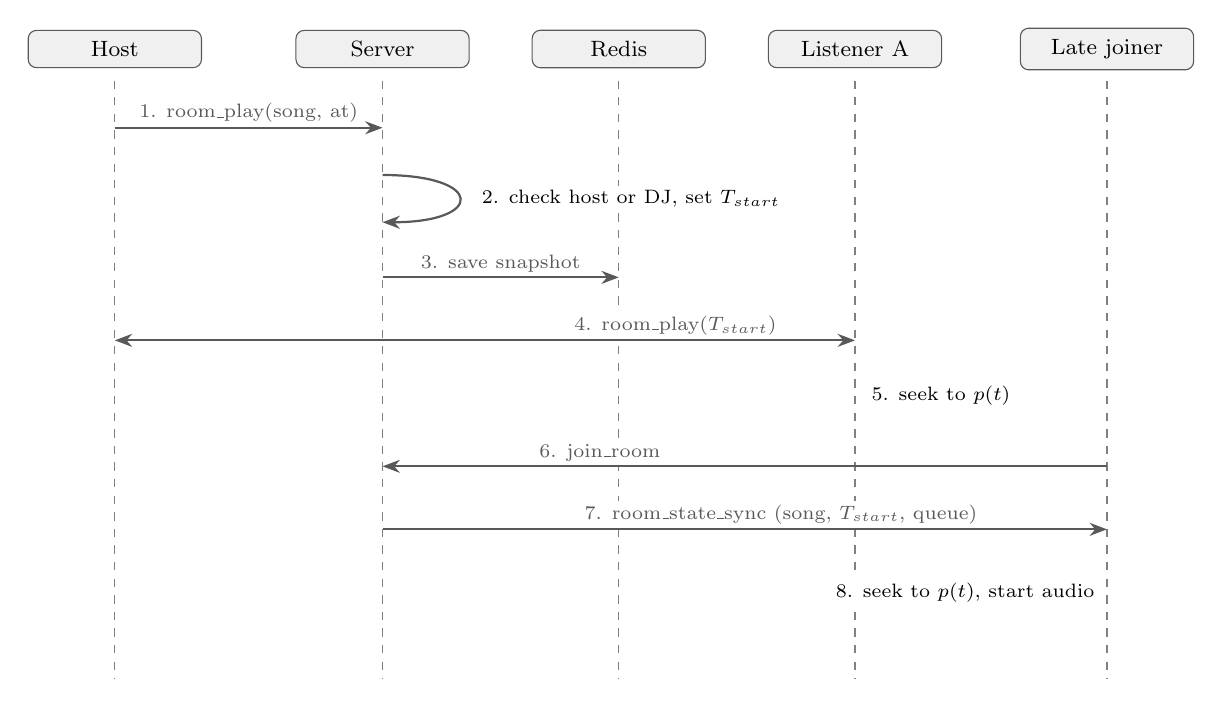
\begin{tikzpicture}[font=\footnotesize]
\foreach \x/\name in {0/Host, 3.4/Server, 6.4/Redis, 9.4/Listener A, 12.6/Late joiner}{
  \node[blk=gray, minimum width=2.2cm] at (\x,0) {\name};
  \draw[dashed, gray] (\x,-0.4) -- (\x,-8);
}
\draw[flow] (0,-1.0) -- (3.4,-1.0) node[midway, above, lab]{1. room\_play(song, at)};
\draw[flow] (3.4,-1.6) .. controls (4.7,-1.6) and (4.7,-2.2) .. (3.4,-2.2);
\node[lab, anchor=west] at (4.6,-1.9) {2. check host or DJ, set $T_{start}$};
\draw[flow] (3.4,-2.9) -- (6.4,-2.9) node[midway, above, lab]{3. save snapshot};
\draw[flow] (3.4,-3.7) -- (0,-3.7);
\draw[flow] (3.4,-3.7) -- (9.4,-3.7) node[pos=0.62, above, lab]{4. room\_play($T_{start}$)};
\node[lab, anchor=west] at (9.55,-4.4) {5. seek to $p(t)$};
\draw[flow] (12.6,-5.3) -- (3.4,-5.3) node[pos=0.7, above, lab]{6. join\_room};
\draw[flow] (3.4,-6.1) -- (12.6,-6.1) node[pos=0.55, above, lab]{7. room\_state\_sync (song, $T_{start}$, queue)};
\node[lab, anchor=east] at (12.5,-6.9) {8. seek to $p(t)$, start audio};
\end{tikzpicture}}
\caption{Message flow for a host play action (steps 1 to 5) and a late join (steps 6 to 8).}
\label{fig:sequence}
\end{figure}

\subsection{How the scenarios map onto existing parts}
\begin{table}[htbp]
\centering
\caption{What each scenario needs and which part of Dhuno provides it.}
\label{tab:mapping}
\footnotesize
\begin{tabularx}{\textwidth}{@{}>{\raggedright\arraybackslash}X>{\raggedright\arraybackslash}X l@{}}
\toprule
\textbf{Need} & \textbf{Dhuno component} & \textbf{Status} \\
\midrule
Everyone on the same second & Reference instant $T_{start}$ and client-side seek & \partialstatus{} (assumes clocks agree) \\
Only the performer or host controls playback & Server-side check, DJ mode & \done \\
Latecomer or dropped phone catches up & \texttt{room\_state\_sync}, Redis snapshot & \done \\
Find a room nearby & GeoJSON and \texttt{2dsphere} index, 1 km radius & \done \\
Performer's own tracks & Artist upload to Cloudinary & \done \\
Music without internet & IndexedDB downloads & \partialstatus{} \\
Connect nearby devices without internet & Nearby mode (Section~\ref{sec:nearby}) & \planned \\
\bottomrule
\end{tabularx}
\end{table}

% ======================================================================
\section{What is implemented so far}\label{sec:done}
% ======================================================================
The system is a working full-stack application, written in TypeScript on both sides. The
frontend uses React 19, Vite, Tailwind CSS 4 and React Router 7. The backend uses
Node.js, Express 5, Socket.IO 4 and Mongoose, with Redis through ioredis and Cloudinary
for media. Table~\ref{tab:status} lists the features and their status.

\footnotesize
\begin{longtable}{@{}>{\raggedright\arraybackslash}p{3.8cm}>{\raggedright\arraybackslash}p{9.4cm}l@{}}
\caption{Implementation status.}\label{tab:status}\\
\toprule
\textbf{Area} & \textbf{Details} & \textbf{Status} \\
\midrule
\endfirsthead
\toprule
\textbf{Area} & \textbf{Details} & \textbf{Status} \\
\midrule
\endhead
\bottomrule
\endfoot
Accounts and sessions & Sign-up, login, JWT in an httpOnly cookie or bearer header, bcrypt hashing, profile editing & \done \\
Two-factor and recovery & E-mailed one-time codes for 2FA and password reset, backup codes, per-route rate limits & \done \\
Google sign-in & Works, but the server trusts the profile sent by the client instead of verifying Google's ID token & \partialstatus \\
Player and library & One global audio element, playlists with drag-and-drop ordering, liked songs, recently played & \done \\
Search and trending & Case-insensitive title and artist search (20 results), trending list cached for 5 minutes & \done \\
Rooms & Create, join, leave, public or private, location filter within 1 km & \done \\
Control and roles & Host or DJ only playback, DJ mode and assignment, host promotion when the host leaves & \done \\
Resilience & Full state sync on join, Redis room snapshot (1 h), presence heartbeat (90 s), restore after restart & \done \\
Room social features & Chat, reactions, shared queue with reorder and remove, vote to skip & \done \\
Artist workspace & Upload songs and cover art (25 MB limit, MIME whitelist), artist playlists, dashboard & \done \\
Artist clips and analytics & Clip pages and analytics pages exist, depth of features still growing & \partialstatus \\
Themes and notifications & Theme picker, in-app notifications; mood-aware themes not started & \partialstatus \\
Offline downloads & Songs saved as blobs in IndexedDB and played from there. The app shell is not cached, so the page itself still needs a network to open & \partialstatus \\
Deployment & Docker images for both apps, Nginx static hosting, GitHub Actions deploying the backend to Azure Web App & \done \\
Clock-offset compensation & Not implemented, see Section~\ref{sec:sync} & \planned \\
Automated tests and load tests & Scenarios are checked by hand; no automated suite yet & \planned \\
Background job queue & BullMQ is a dependency but unused; e-mail is sent inline & \planned \\
\end{longtable}
\normalsize

% ======================================================================
\section{Where the system falls short of the use cases}\label{sec:gaps}
% ======================================================================
\begin{table}[htbp]
\centering
\caption{Gaps between the use cases and the current implementation.}
\label{tab:gaps}
\footnotesize
\begin{tabularx}{\textwidth}{@{}l>{\raggedright\arraybackslash}X>{\raggedright\arraybackslash}X@{}}
\toprule
\textbf{Gap} & \textbf{Why it matters} & \textbf{Planned fix} \\
\midrule
G1 Clock offset not compensated & Listeners drift apart, phones used as speakers produce echo & NTP-style handshake and drift threshold \\
G2 Device output latency differs & Bluetooth headphones add delay, so the same instant sounds different per device & Per-device calibration \\
G3 Needs internet and a server & Cars and crowded venues have poor connectivity & Offline nearby mode \\
G4 One server instance, in-memory state & A large audience cannot be served by one process & Socket.IO Redis adapter, several instances, load tests \\
G5 Only stored tracks & A live band cannot be streamed; a DJ set from uploaded tracks can & Live audio ingest, later \\
G6 App shell not cached & The app cannot open offline even if songs are downloaded & Service worker \\
G7 Google token not verified server-side & A forged profile could claim an account & Verify the ID token on the server \\
G8 No measurements & Claims about sync quality cannot yet be proven & Evaluation plan (Section~\ref{sec:eval}) \\
\bottomrule
\end{tabularx}
\end{table}

\subsection{The most important gap: synchronization}\label{sec:sync}
The server computes $T_{start}$ from \emph{its own} clock, but each listener's browser
evaluates $p(t)$ with the \emph{local} clock (\texttt{Date.now()}). The formulas therefore
assume that server and client clocks agree. A phone whose clock is two seconds off will
play two seconds off, with no way to notice. Phone clocks are usually corrected by the
network, which is why the approach works for casual use, but that is not guaranteed, and
the in-person scenarios depend on it much more.

For headphone listening (UC1, UC4) some drift is tolerable. For several phones acting as
speakers in one room (UC3), a difference of a few tens of milliseconds is heard as echo.
The report's own scope statement excludes sample-accurate alignment, and we agree it is not
needed, but it does need to be \emph{better than now and measured}.

% ======================================================================
\section{Future work}\label{sec:future}
% ======================================================================
\subsection{Clock-offset and latency compensation}
Each client estimates the offset $\theta$ between its clock and the server clock with four
timestamps, as in the Network Time Protocol~\cite{ntp}: its request time $t_0$, the server's receive and send times $t_1$ and $t_2$, and
its own receive time $t_3$:
\begin{equation}
  \theta = \frac{(t_1 - t_0) + (t_2 - t_3)}{2}.
\end{equation}
It repeats the exchange several times and keeps the estimate from the shortest round trip,
which is the least disturbed by queuing. The position then becomes
\begin{equation}
  p(t) = \frac{t + \theta - T_{start}}{1000} + \lambda,
\end{equation}
where $\lambda$ is a per-device correction for audio output delay, for example when
Bluetooth headphones are used. The client seeks only when $\left|p(t) - \text{currentTime}\right| > \delta$,
for a threshold $\delta$ tuned by experiment, so tiny differences do not cause audible jumps.
Cristian's algorithm~\cite{cristian} is a simpler variant that we can use as a baseline.

\subsection{Offline nearby mode on the web}\label{sec:nearby}
For the car and room scenarios, devices need to sync with no internet. Dhuno is a website,
and a browser cannot do some of the obvious things. Web Bluetooth only lets a page
connect \emph{out} to a device; a page cannot advertise a room or accept connections, and
iOS Safari does not support it. Browsers also have no API for Wi-Fi Direct or for scanning
nearby devices. A native app wrapper would remove these limits, but it changes the product
from a website to an app, so we treat it as a later option.

The web-only design uses a local network that needs no internet (a phone hotspot or a
router) and WebRTC data channels~\cite{webrtc,rtcdc} between the devices (Figure~\ref{fig:nearby}).
\begin{enumerate}
  \item \textbf{Offline app shell.} A service worker caches the app so it opens with no
        network. The IndexedDB song store already exists.
  \item \textbf{Local network.} All devices join the same hotspot or router. No internet is
        required.
  \item \textbf{QR-code pairing.} Without a signalling server, devices exchange the WebRTC
        connection offer and answer by scanning each other's QR codes. After that, the
        browsers talk directly.
  \item \textbf{Local room engine.} The host's device runs the same room logic as the
        Socket.IO gateway (same events: play, pause, seek, queue, join) and sends them over
        the data channels. A \texttt{Transport} interface lets the UI use either Socket.IO
        online or data channels offline.
  \item \textbf{File sharing.} Songs a guest lacks are sent from the host in chunks over the
        data channel and stored in IndexedDB before playback.
  \item \textbf{Clock sync.} The ping-pong exchange of Section~\ref{sec:sync} runs over the
        data channel, so offline playback is scheduled as ``play X at time $T$''.
\end{enumerate}
Audio is never streamed live over the link. Every device plays its own local copy,
started at the agreed time.

\textbf{Limits we expect.} Pairing is manual, so there is no automatic list of nearby
rooms. Some phones and routers block device-to-device traffic (client isolation), which we
must test on real hotspots. Browsers may pause audio or connections when the screen locks,
especially on iOS. Each guest is a separate peer connection to the host, so the group
size is small; we expect a handful of guests per host and will measure the real limit.

\begin{figure}[htbp]
\centering
\resizebox{\linewidth}{!}{%
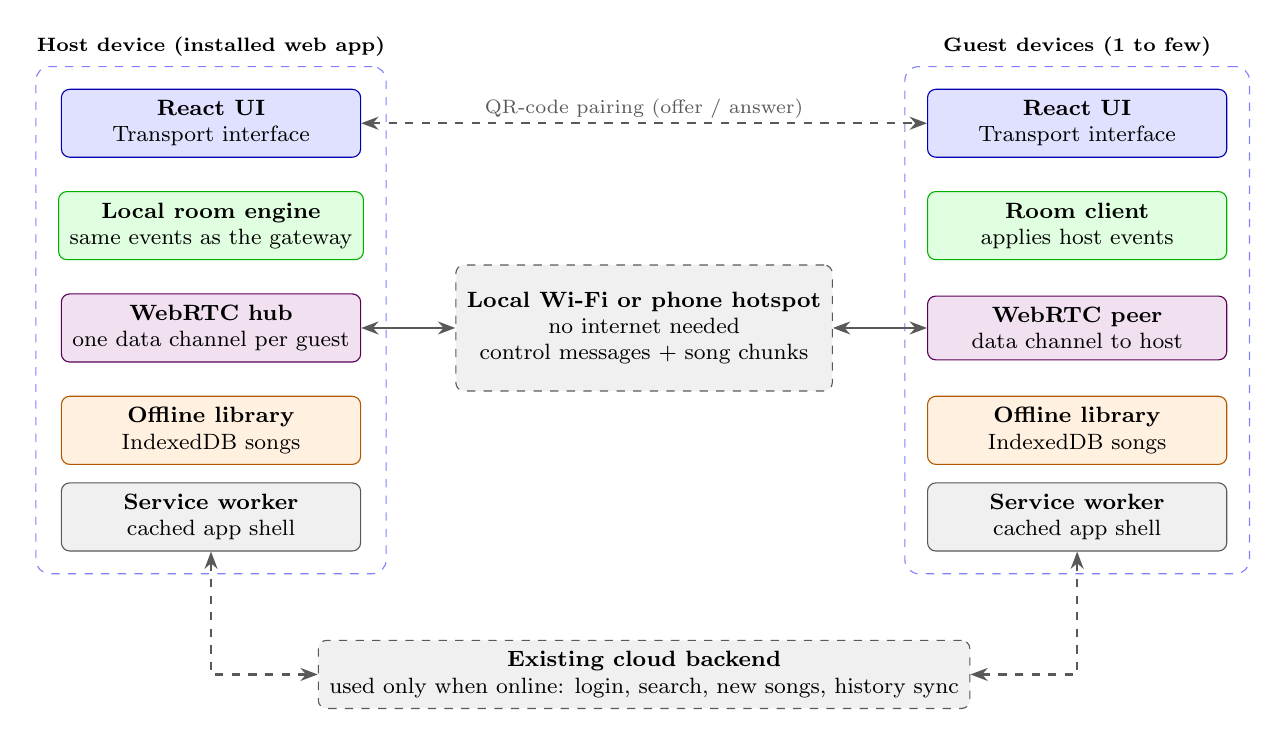
\begin{tikzpicture}[font=\footnotesize]
% host
\node[blk=blue, minimum width=3.8cm] (h1) at (2.0,3.6) {\textbf{React UI}\\Transport interface};
\node[blk=green, minimum width=3.8cm] (h2) at (2.0,2.3) {\textbf{Local room engine}\\same events as the gateway};
\node[blk=violet, minimum width=3.8cm] (h3) at (2.0,1.0) {\textbf{WebRTC hub}\\one data channel per guest};
\node[blk=orange, minimum width=3.8cm] (h4) at (2.0,-0.3) {\textbf{Offline library}\\IndexedDB songs};
\node[blk=gray, minimum width=3.8cm] (h5) at (2.0,-1.4) {\textbf{Service worker}\\cached app shell};
\begin{scope}[on background layer]
\node[grp=blue, fit=(h1)(h2)(h3)(h4)(h5), label={[font=\scriptsize\bfseries]above:Host device (installed web app)}] {};
\end{scope}
% guest
\node[blk=blue, minimum width=3.8cm] (g1) at (13.0,3.6) {\textbf{React UI}\\Transport interface};
\node[blk=green, minimum width=3.8cm] (g2) at (13.0,2.3) {\textbf{Room client}\\applies host events};
\node[blk=violet, minimum width=3.8cm] (g3) at (13.0,1.0) {\textbf{WebRTC peer}\\data channel to host};
\node[blk=orange, minimum width=3.8cm] (g4) at (13.0,-0.3) {\textbf{Offline library}\\IndexedDB songs};
\node[blk=gray, minimum width=3.8cm] (g5) at (13.0,-1.4) {\textbf{Service worker}\\cached app shell};
\begin{scope}[on background layer]
\node[grp=blue, fit=(g1)(g2)(g3)(g4)(g5), label={[font=\scriptsize\bfseries]above:Guest devices (1 to few)}] {};
\end{scope}
% network
\node[blk=gray, dashed, minimum width=4.2cm, minimum height=1.6cm] (net) at (7.5,1.0)
  {\textbf{Local Wi-Fi or phone hotspot}\\no internet needed\\control messages + song chunks};
\draw[flow2] (h3.east) -- (net.west);
\draw[flow2] (net.east) -- (g3.west);
\draw[flow2, dashed] (h1.east) -- (g1.west) node[midway, above, lab]{QR-code pairing (offer / answer)};
% cloud
\node[blk=gray, dashed, minimum width=7cm] (cl) at (7.5,-3.4) {\textbf{Existing cloud backend}\\used only when online: login, search, new songs, history sync};
\draw[flow2, dashed] (h5.south) |- (cl.west);
\draw[flow2, dashed] (g5.south) |- (cl.east);
\end{tikzpicture}}
\caption{Proposed offline nearby mode for the web: PWA, local network, WebRTC data channels
and QR-code pairing.}
\label{fig:nearby}
\end{figure}

\textbf{Native option.} If the project later becomes an installed app (for example by
wrapping the web app with Capacitor), Bluetooth LE can be used for automatic discovery and
small control messages, and Wi-Fi Direct or Nearby Connections for copying song files.
Bluetooth LE is too slow to carry audio, so the same rule applies: devices share files
first, then play locally on a shared clock.

\subsection{Concert mode}
A silent concert has one host and a large audience, so the single-instance design must grow
(Figure~\ref{fig:concert}). The plan is to use the Socket.IO Redis adapter so that several
gateway instances share rooms through Redis, to place a load balancer in front, and to run
load tests that measure the number of listeners per instance before latency grows. Other
items are a larger audience view for the host, a reaction wall, and, later, live audio
ingest so a performer can be heard live and not only from uploaded tracks.

\begin{figure}[htbp]
\centering
\resizebox{0.95\linewidth}{!}{%
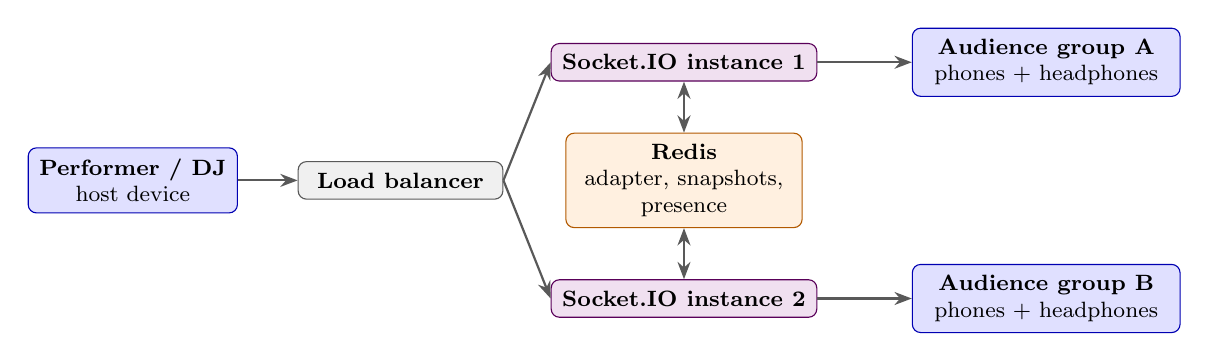
\begin{tikzpicture}[font=\footnotesize]
\node[blk=blue, minimum width=2.6cm] (host) at (0,1.5) {\textbf{Performer / DJ}\\host device};
\node[blk=gray, minimum width=2.6cm] (lb) at (3.4,1.5) {\textbf{Load balancer}};
\node[blk=violet, minimum width=3.2cm] (i1) at (7.0,3.0) {\textbf{Socket.IO instance 1}};
\node[blk=violet, minimum width=3.2cm] (i2) at (7.0,0.0) {\textbf{Socket.IO instance 2}};
\node[blk=orange, minimum width=3.0cm] (rd) at (7.0,1.5) {\textbf{Redis}\\adapter, snapshots,\\presence};
\node[blk=blue, minimum width=3.4cm] (a1) at (11.6,3.0) {\textbf{Audience group A}\\phones + headphones};
\node[blk=blue, minimum width=3.4cm] (a2) at (11.6,0.0) {\textbf{Audience group B}\\phones + headphones};
\draw[flow] (host)--(lb);
\draw[flow] (lb.east)--(i1.west); \draw[flow] (lb.east)--(i2.west);
\draw[flow] (i1)--(a1); \draw[flow] (i2)--(a2);
\draw[flow2] (i1)--(rd); \draw[flow2] (rd)--(i2);
\end{tikzpicture}}
\caption{Proposed scaling for a large audience. Rooms are shared across instances through Redis.}
\label{fig:concert}
\end{figure}

\subsection{Speaker-array mode}
For UC3, several phones in one room can play the same track as a distributed speaker
system. Beyond tight synchronization, an extra idea is to let the host give each phone a
role (left, right, or bass-heavy) so the room sounds fuller. This depends on the
sync work in Section~\ref{sec:sync} and is the most experimental item here.

\subsection{Other planned work}
These items come from the main report and remain on the list.
\begin{itemize}
  \item \textbf{Security.} Verify Google ID tokens on the server, replace the wildcard
        cross-origin header on the static host with the known frontend origin, and review
        the large request-body limit.
  \item \textbf{Search.} Indexed, typo-tolerant, ranked search with escaped input and cached
        popular queries.
  \item \textbf{Recommendations.} Popularity and content-based suggestions from plays,
        likes and room activity, then collaborative filtering and recommended rooms.
  \item \textbf{Background jobs.} Move e-mail and clean-up into BullMQ workers.
  \item \textbf{Testing.} Automated unit and integration tests, end-to-end tests with
        several simulated clients, and load tests.
  \item \textbf{Interaction.} Voice commands, mood-aware themes, invitation links.
\end{itemize}

% ======================================================================
\section{Evaluation plan}\label{sec:eval}
% ======================================================================
The main report claims no latency figures because none were measured. The use cases make
measurement necessary. Table~\ref{tab:eval} lists what we will measure. The targets are
hypotheses to be tuned from the first results, not promises.

\begin{table}[htbp]
\centering
\caption{Planned measurements.}
\label{tab:eval}
\footnotesize
\begin{tabularx}{\textwidth}{@{}>{\raggedright\arraybackslash}p{3.6cm}>{\raggedright\arraybackslash}X>{\raggedright\arraybackslash}p{3.2cm}@{}}
\toprule
\textbf{Metric} & \textbf{How we measure it} & \textbf{Target} \\
\midrule
Start-time spread between listeners & Play a click track on several phones and record all of them with a separate recorder. Compare the click onsets. Also log each client's expected versus actual position. & Tens of milliseconds or better, compared before and after clock compensation \\
Late-join convergence & Time from \texttt{join\_room} to audio at the correct position. & Under a few seconds \\
Reconnection recovery & Drop and restore a client's connection, and restart the server, then check the room state. & State restored with no manual step \\
Capacity per instance & Simulated Socket.IO clients joining one room until event latency grows. & Find the limit, then raise it with the Redis adapter \\
Offline pairing and transfer & QR pairing success rate, and transfer time per song on a hotspot and on a router. & Reliable on at least two phone models \\
\bottomrule
\end{tabularx}
\end{table}

% ======================================================================
\section{Roadmap}\label{sec:roadmap}
% ======================================================================
We propose doing the work in the order that unlocks the use cases soonest. Synchronization
accuracy and measurement come first, because every in-person scenario depends on them.

\begin{figure}[htbp]
\centering
\resizebox{\linewidth}{!}{%
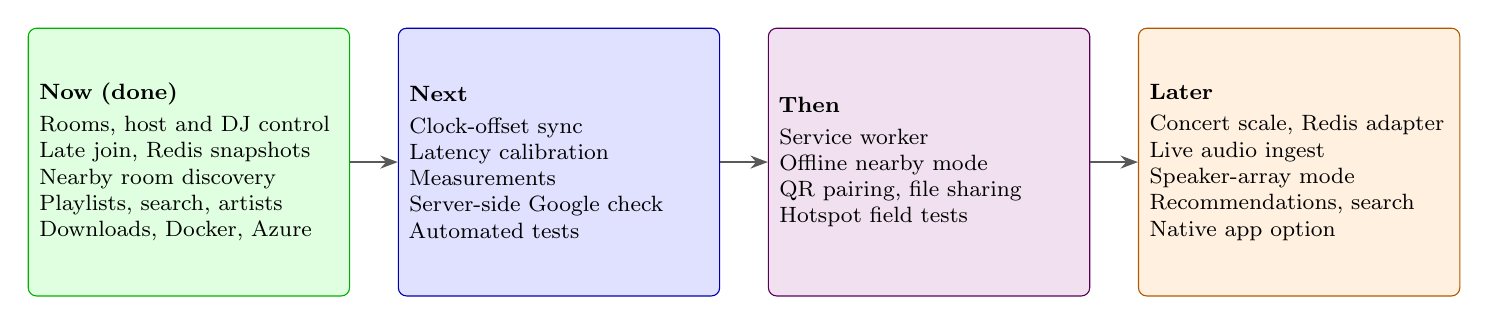
\begin{tikzpicture}[font=\footnotesize]
\hyphenpenalty=10000 \exhyphenpenalty=10000
\node[blk=green, text width=3.8cm, align=left, minimum height=3.4cm, anchor=north west] (r1) at (0,0)
  {\textbf{Now (done)}\\[2pt]
   Rooms, host and DJ control\\
   Late join, Redis snapshots\\
   Nearby room discovery\\
   Playlists, search, artists\\
   Downloads, Docker, Azure};
\node[blk=blue, text width=3.8cm, align=left, minimum height=3.4cm, anchor=north west] (r2) at (4.7,0)
  {\textbf{Next}\\[2pt]
   Clock-offset sync\\
   Latency calibration\\
   Measurements\\
   Server-side Google check\\
   Automated tests};
\node[blk=violet, text width=3.8cm, align=left, minimum height=3.4cm, anchor=north west] (r3) at (9.4,0)
  {\textbf{Then}\\[2pt]
   Service worker\\
   Offline nearby mode\\
   QR pairing, file sharing\\
   Hotspot field tests};
\node[blk=orange, text width=3.8cm, align=left, minimum height=3.4cm, anchor=north west] (r4) at (14.1,0)
  {\textbf{Later}\\[2pt]
   Concert scale, Redis adapter\\
   Live audio ingest\\
   Speaker-array mode\\
   Recommendations, search\\
   Native app option};
\draw[flow] (r1.east) -- (r2.west);
\draw[flow] (r2.east) -- (r3.west);
\draw[flow] (r3.east) -- (r4.west);
\end{tikzpicture}}
\caption{Proposed order of work.}
\label{fig:roadmap}
\end{figure}

% ======================================================================
\section{Conclusion}
% ======================================================================
Dhuno started from a simple observation: people want to hear music together, and the
hardware and noise that usually come with that are a poor fit for concerts, cars and small
parties. A synchronized room model, with a host who controls playback and every phone
playing its own copy, addresses all three. The current release already delivers the room
model, host and DJ control, late join, nearby discovery, an artist workspace and offline
downloads, and it serves remote friends well.

The in-person scenarios ask for more than the release gives: tighter, measured
synchronization, the ability to work without internet, and capacity for large audiences.
We have identified these gaps, designed a web-only way to close them, and ordered the work
so that measurement comes first. Completing it would turn Dhuno from a way to listen
together at a distance into a way to share a sound system among everyone in the room.

% ======================================================================
\begin{thebibliography}{99}
\bibitem{ws} I.~Fette and A.~Melnikov, ``The WebSocket Protocol,'' RFC 6455, IETF, Dec. 2011.
\bibitem{ntp} D.~Mills, J.~Martin, J.~Burbank and W.~Kasch, ``Network Time Protocol Version 4: Protocol and Algorithms Specification,'' RFC 5905, IETF, Jun. 2010.
\bibitem{cristian} F.~Cristian, ``Probabilistic clock synchronization,'' \emph{Distributed Computing}, vol.~3, no.~3, pp.~146--158, 1989.
\bibitem{socketio} Socket.IO Documentation, v4. [Online]. Available: https://socket.io/docs/v4/
\bibitem{mongo} MongoDB Inc., ``2dsphere indexes,'' MongoDB Manual. [Online]. Available: https://www.mongodb.com/docs/manual/core/2dsphere/
\bibitem{redis} Redis Documentation. [Online]. Available: https://redis.io/docs/
\bibitem{webrtc} W3C, ``WebRTC 1.0: Real-Time Communication Between Browsers,'' W3C Recommendation, Jan. 2021.
\bibitem{rtcdc} R.~Jesup, S.~Loreto and M.~Tuexen, ``WebRTC Data Channels,'' RFC 8831, IETF, Jan. 2021.
\bibitem{jam} ``Spotify launches Jam, a real-time collaborative playlist controlled by up to 32 people,'' \emph{TechCrunch}, Sep. 26, 2023.
\bibitem{main} N.~Agrawal, K.~Vanshaj and P.~K.~Goyal, ``Dhuno: A Real-Time Synchronized Music Streaming Platform with Host-Controlled Listening Rooms,'' B.Tech project report, IIIT Bhubaneswar, Oct. 2026.
\end{thebibliography}

\end{document}
